\begin{figure*}[t]
  \centering
  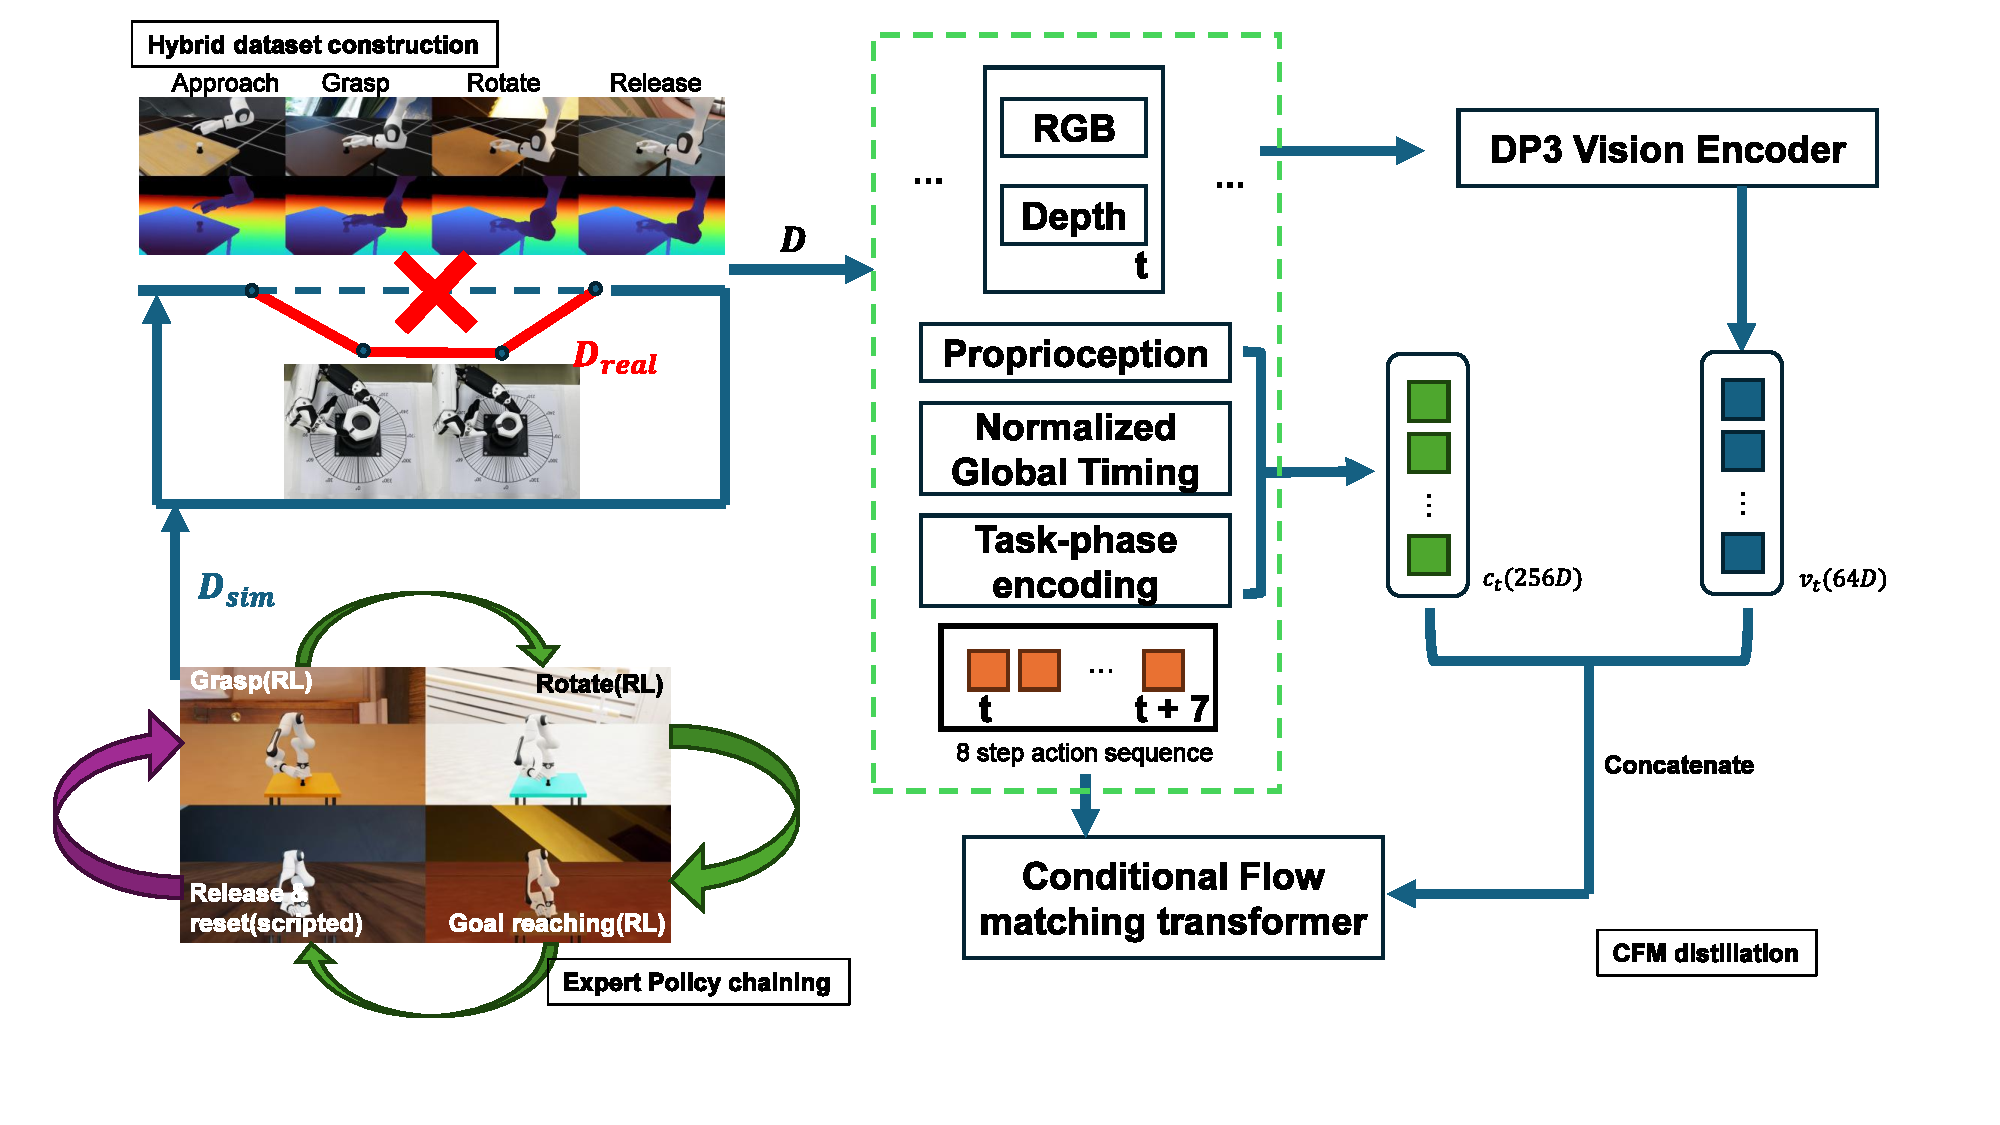
\includegraphics[width=0.90\textwidth]{mainpipeline.pdf}
  \caption{Detailed NUTS pipeline. An RL teacher is repeatedly rolled out with
    a scripted policy to construct cyclic threading demonstrations in
    simulation; together, they form the hybrid teacher. During real-world
    replay, human corrections replace flawed trajectory segments from grasp
    through release, forming a mixed simulation and real-world dataset. The
    conditional flow-matching student takes a 64-D visual feature extracted by
    a DP3 vision encoder from RGB-D observations and a 256-D state feature
    comprising proprioception, timing, and phase encodings, and predicts an
    eight-step action chunk.}
  \label{fig:main_pipeline}
\end{figure*}
